\chapter{Display modes: box and tree}
\label{chap:boxNtree}

\begin{figure}
\begin{center}
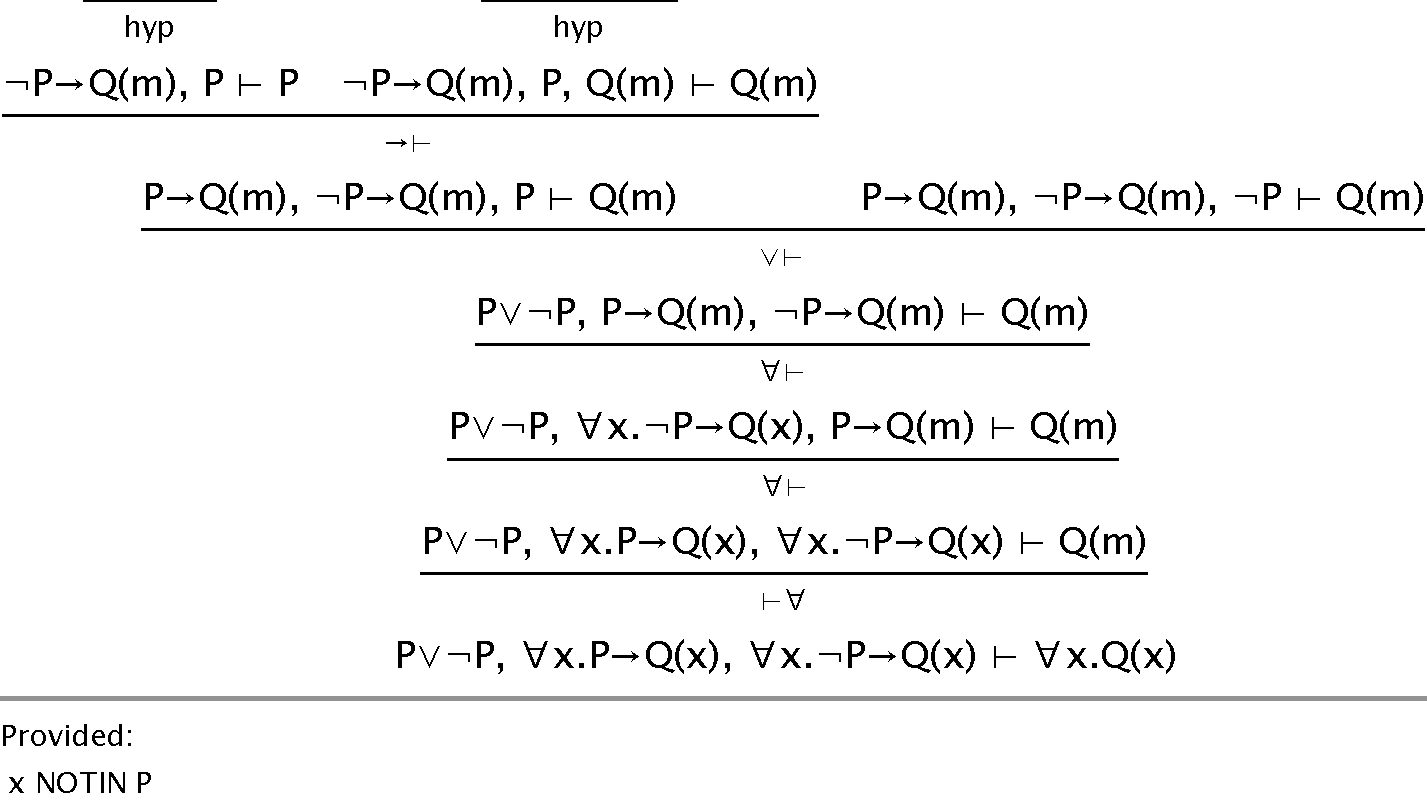
\includegraphics[scale=0.5]{pics/sampletree}
\caption{A sample proof attempt, shown as a tree}
\label{fig:sampletree}
\end{center}
\end{figure}

\begin{figure}
\begin{center}
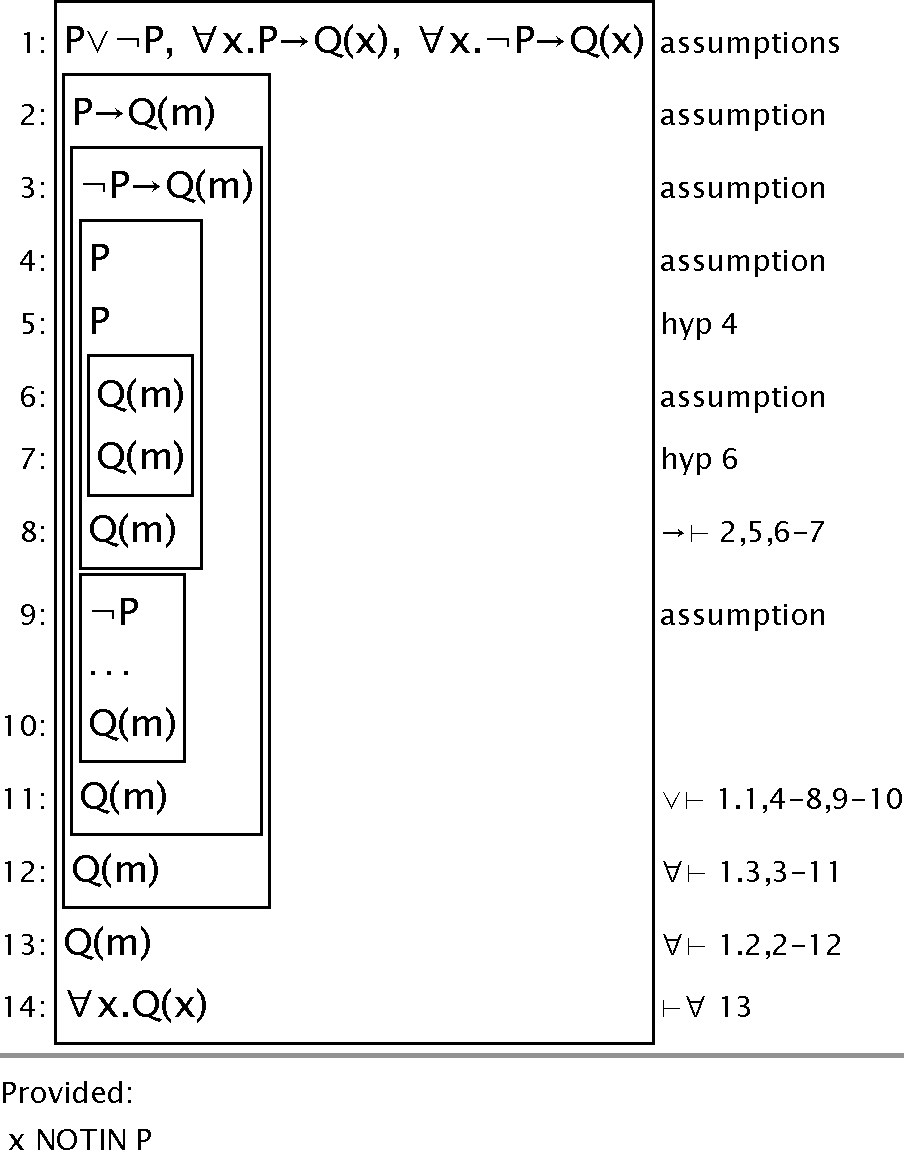
\includegraphics[scale=0.5]{pics/sampleboxNline}
\caption{A sample proof attempt, shown as box-and-line}
\label{fig:sampleboxNline}
\end{center}
\end{figure}

\begin{figure}
\begin{center}
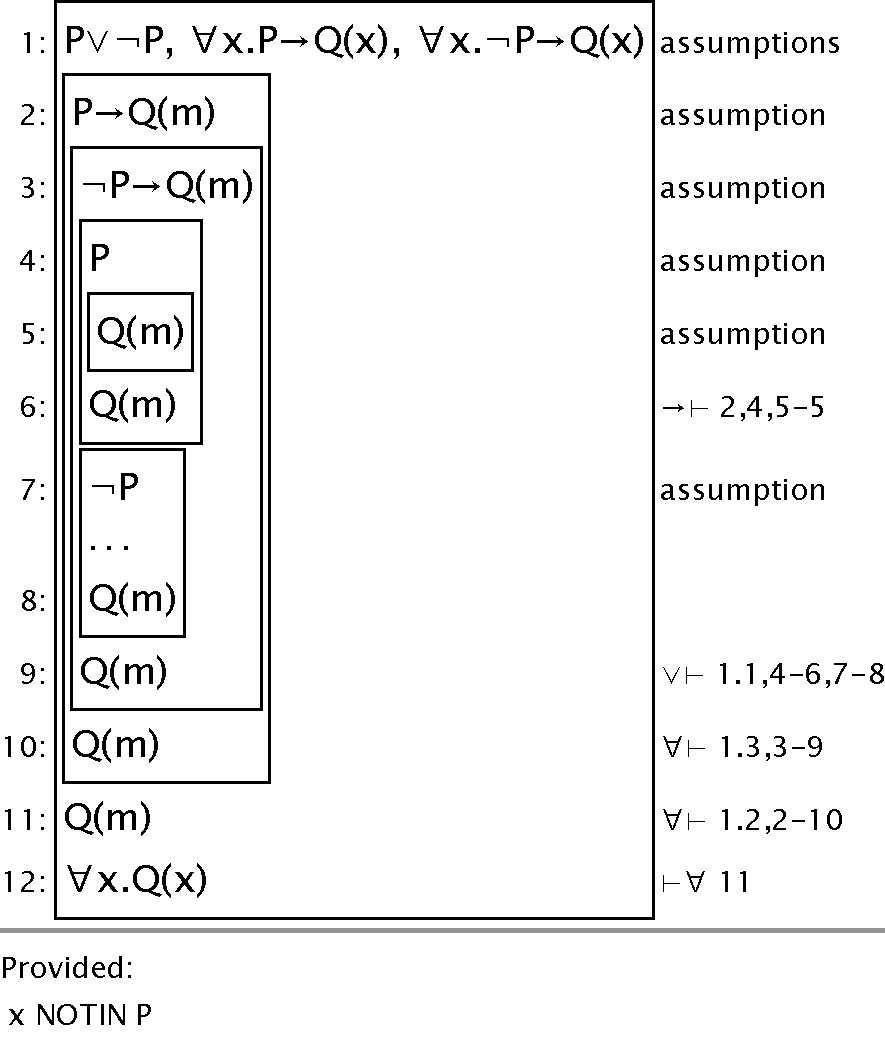
\includegraphics[scale=0.5]{pics/sampleboxNlinehiddenhyp}
\caption{A sample proof attempt, shown as box-and-line, with hidden \texttt{hyp} steps}
\label{fig:sampleboxNlinehiddenhyp}
\end{center}
\end{figure}

\Figref{sampletree} shows a sample proof attempt in the intuitionistic single-conclusion sequent calculus (see \texttt{examples/SCS.jt} and \chapref{sequentvariations}). It's a large tree, partly because the hypotheses are written out many times, once in each sequent in which they occur. The same proof attempt in box-and-line form is shown in \figref{sampleboxNline}: it's much narrower and, because it's essentially one-dimensional, easier to navigate. It shows exactly the same steps as the tree and is produced by a very simple algorithm: 
\begin{itemize}
\item to list a node list its antecedent nodes, then the consequent of the sequent;
\item if a node has more hypothesis formulae than its parent, show it as a box with the additional hypotheses on a line labelled `assumptions';
\item link a conclusion to its antecedents by giving their line number (or, if a box, their starting and finishing line numbers);
\item precede tips (unclosed nodes) with a line of three dots.
\end{itemize}
The algorithm saves a great deal of screen space. When a problem sequent has more than a few short hypotheses the tree will often be very wide, impossible to view in one piece. The box-and-line display is still readable, and it's easier to find your way around because you only have to go up and down.

The simple algorithm is only just the beginning ...

\section{Hiding \textsc{identity} steps}

There is still unnecessary business in \figref{sampleboxNline}. Line 5, for example, is proved by \texttt{hyp}. That rule, in the SCS encoding, is
\begin{quote}\tt\small
RULE hyp(A) INFER A ⊦ A
\end{quote}
It makes sense in the tree, but in the box-and-line version it's little more than an indirection. Line 8, for example, appeals to line 5 which appeals immediately and identically to line 4. When the r\^{o}le of \texttt{hyp} is declared to Jape
\begin{quote}\tt\small
STRUCTURERULE IDENTITY hyp
\end{quote}
and the \texttt{hidehyp} variable is set to \texttt{true} (its default value), then the picture changes to \figref{sampleboxNlinehiddenhyp}. The old line 8 is now line 6 and refers directly to the assumption on line 3. The proof is more compact, and easier to read. There's still tedious repetition of the conclusion $Q(m)$ in lines 5-6 and 8-11, but that is inevitable in this calculus, where left-hand-side rules transform hypotheses and copy the conclusion. \Chapref{ItL} shows how a Natural Deduction calculus, without left-hand rules, can avoid such repetition.

An \textsc{identity} step can still appear in a box-and-line proof if it is the last line of a box which has more than two lines, or the assumption line isn't a single formula which is the same as the last line.

\begin{figure}
\begin{center}
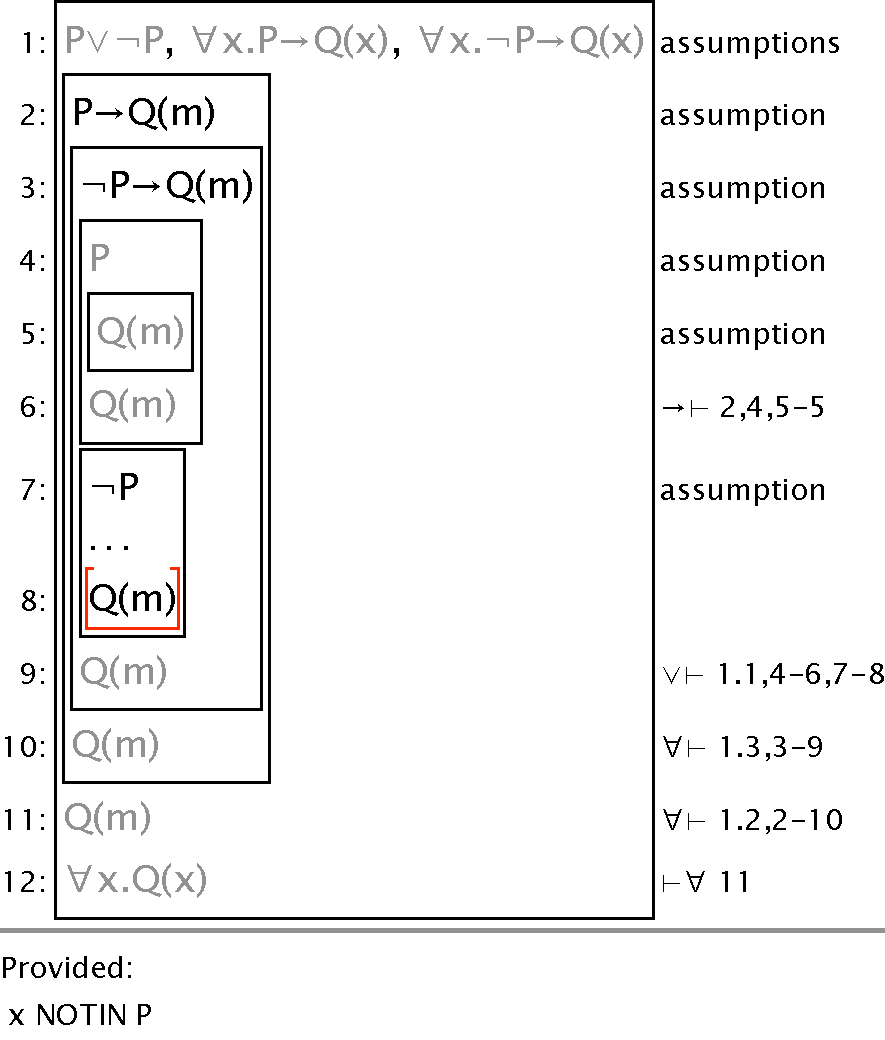
\includegraphics[scale=0.5]{pics/sampleboxNlinegreyed}
\caption{In the box-and-line presentation not all accessible formulae are usable}
\label{fig:sampleboxNlinegreyed}
\end{center}
\end{figure}

\begin{figure}
\centering
\subfigure[A bifurcated tree]{\centering
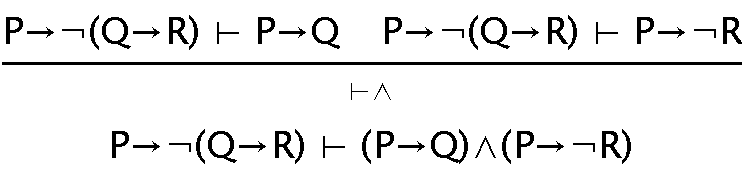
\includegraphics[scale=0.5]{pics/treebifurcated}\label{fig:treebifurcated}}
\qquad
\subfigure[Box-and-line presentation of a bifurcated tree]{\centering
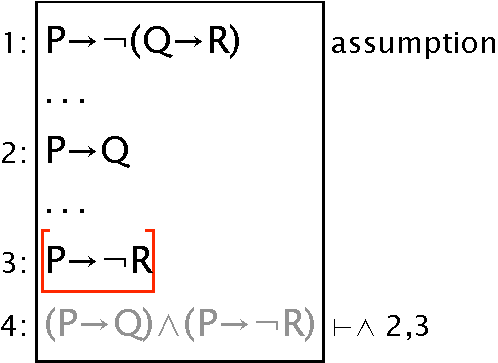
\includegraphics[scale=0.5]{pics/boxNlinebifurcated}\label{fig:boxNlinebifurcated}}
\caption{Bifurcation also causes presentation problems}
\end{figure}

\section{The tree is still there}

In \figref{sampleboxNlinehiddenhyp}, according to the rules of box-and-line proof presentation, line 8 can appeal to the assumptions on line 1, 2, 3 and 7 (it can't use line 9-12 because they are below it; it can't use lines 4-6 because they are in a box). But in the tree only $P->Q(m)$, $!P->Q(m)$ and $!P$ --- that is, lines 2, 3 and 7 --- are available. If you select the conclusion on line 8 Jape greys out all the formulae that can't be used: see \figref{sampleboxNlinegreyed}.

The effect in \figref{sampleboxNlinegreyed} is produced by left-hand rules that use up hypotheses. When a rule bifurcates the proof there are other problems. In \figref{boxNlinebifurcated}, for example, the formula on line 2 can't be selected as a hypothesis to help prove the conclusion on line 3, which breaks the normal rules of box-and-line proofs: it isn't greyed out, though, because it is possible to move the conclusion selection from line 3 to line 2. The solution to this problem is presented in \chapref{I2L}.

\section{That's not all}

Box-and-line mode, produced by setting variable \texttt{displaystyle} to \texttt{true}, can be used as an abbreviated mode of presentation of any tree proof, if you are prepared to live with the deficiencies described above. In Natural Deduction logics, without left-hand rules, it's possible to do much more, using hidden \textsc{cut} steps to produce an approximation to forward reasoning from the hypotheses (\chapref{ItL}) or, at some considerable effort, an accurate depiction (\chapref{I2L}).
